\documentclass[beamer, table,xcdraw]{beamer}

\usepackage[T1]{fontenc}
\usepackage[spanish, mexico]{babel}
\usepackage{geometry} % Add this line
\usepackage{graphicx}
\usepackage{verbatim}
\usepackage{lipsum}
\usepackage{enumitem}
\usepackage{subfig}
\usepackage{multicol}
\usepackage{multirow}
\usepackage{fancyhdr}
\usepackage{hyperref}
\usepackage{tcolorbox}
\usepackage{paracol}
\usepackage{amsmath}
\usepackage{amssymb}
\usepackage{tikz}
\usetikzlibrary{positioning,shadows,backgrounds,automata,arrows,arrows.meta}
\usepackage{xcolor}

\definecolor{gluoblue}{HTML}{2e75b5}
\definecolor{gluoblue2}{HTML}{528DD9}
\definecolor{gluogrisconsola}{HTML}{E7E6E6}
\definecolor{gluogriscaption}{HTML}{44546a}


%\geometry{
%	paperwidth=10in,
%	paperheight=7.5in
%} 

% SIEMRPE EXISTIR\'A UNA CARPETA IMG
\graphicspath{{./img/}}

\setlength{\parskip}{10pt}

% ESPACIADORES
\newcommand{\enter}{\vspace{0.5cm}}
\newcommand{\tab}{\hspace{1cm}}




\usetheme{Copenhagen} % Choose a theme (default, Warsaw, Berlin, etc.)
\usecolortheme{default}
%\titlegraphic{\includegraphics[width=3cm]{cic.png}}



%\documentclass[letterpaper, 12pt]{article} %10pt por default
%\usepackage[paper=a4paper,left=24mm,right=24mm,top=20mm,bottom=20mm]{geometry}

\usepackage[utf8]{inputenc}
\usepackage[spanish]{babel}
\usepackage{geometry}
\usepackage{lipsum} %por si hay que hacer pruebas de como se ver\'ia
\usepackage{graphicx}
%\usepackage{rotating}
\usepackage{paracol}
\usepackage{multicol}
\usepackage[numbers]{natbib}
\usepackage{setspace}
\usepackage{xstring}
\usepackage[table,xcdraw]{xcolor}
\usepackage{xargs}
\usepackage{bbding} %para las palomitas
\usepackage{ragged2e}
\usepackage[hidelinks]{hyperref}
\usepackage{wrapfig}
\usepackage{lscape}
\usepackage{rotating}
\usepackage{epstopdf}
\usepackage{amsmath}
\usepackage{amssymb}
%\usepackage{caption}
%\usepackage{subcaption}
\usepackage{subfig}
%\usepackage[ruled,linesnumbered]{algorithm2e}
\usepackage{listings}
%\usepackage[toc, acronym]{glossaries}
\usepackage{verbatim}
\usepackage{float}
\usepackage{enumitem}
\usepackage{mathrsfs}
\usepackage[makeroom]{cancel}
\usepackage[firstpage=true]{background}


\usepackage{tikz}
\usetikzlibrary{positioning,shadows,backgrounds,automata,arrows,arrows.meta}
%\usetikzlibrary{arrows} %arrows meta
%\usepackage{tikz-qtree} % Easy tree drawing tool
%\tikzset{every tree node/.style={align=center,anchor=north}, level distance=2cm} % Configuration for q-trees


\usepackage[breakable]{tcolorbox}



%Para estilo fancy
%\usepackage{fancyhdr}
%\usepackage{lastpage}fenter
%\pagestyle{fancy}
%\fancyhf{}

%\renewcommand{\headrulewidth}{0pt} %Quitar la l\'inea del encabezado de fancy
%\rfoot{\footnotesize{ P\'agina \thepage \hspace{1pt} de \pageref{LastPage} }}





\decimalpoint
%If you use either the babel or polyglossia package you'll have to change the name for the particular language
%you use with babel or polyglossia.
\addto\captionsspanish{% Replace "english" with the language you use
	\renewcommand{\contentsname}{Tabla de contenido}%
	\renewcommand{\listfigurename}{Lista de figuras}
	\renewcommand{\listtablename}{Lista de tablas}
	\renewcommand{\lstlistlistingname}{Lista de programas}
	\renewcommand{\glossaryname}{Glosario}
	% NOMBRES DE FIGURA, TABLA, ETC.
	%\renewcommand{\thefigure}{Fig.(\arabic{figure})}
	\renewcommand{\figurename}{Figura}
	%\renewcommand{\thetable}{Tab.(\arabic{table})}
	\renewcommand{\tablename}{Tabla}
	%\renewcommand{\theequation}{Eq.(\arabic{equation})}
	\renewcommand{\lstlistingname}{Programa}
}
% RENOMBRAR BIBLIOGRAF\'IA
%\renewcommand{\bibname}{\section{Referencias}}
%\renewcommand{\theenumi}{\Alph{enumi}}
\newcommand{\reftab}[1]{Tab.(\ref{#1})}
\newcommand{\reffig}[1]{Fig.(\ref{#1})}
\newcommand{\refeq}[1]{Ec.(\ref{#1})}
\newcommand{\refexp}[1]{Exp.(\ref{#1})}
\newcommand{\refdef}[1]{Def.(\ref{#1})}
\newcommand{\refsec}[1]{Sec.(\ref{#1})}
\newcommand{\refssec}[1]{Subsec.(\ref{#1})}
\newcommand{\refej}[1]{Ej.(\ref{#1})}
\newcommand{\refprog}[1]{Prog.(\ref{#1})}


% SIEMRPE EXISTIR\'A UNA CARPETA IMG
\graphicspath{{./img/}}

% ESPACIO ENTRE COLUMNAS DE MULTICOL
\setlength{\columnsep}{1cm}

% INTERLINEADO
\setstretch{1} %

% SEPARACI\'ON ENTRE P\'ARRAFOS
\setlength{\parskip}{10pt}

% BORRAR SANGR\'IA EN GENERAL
\setlength\parindent{0pt}


% CONFIGURACI\'ON DE HIPERV\'INCULOS
%\hypersetup{
	%    colorlinks=true,
	%    linkcolor=black,
	%    urlcolor=magenta
	%}

% TAMA\~NO DE LA HOJA
\geometry{
	%headsep= 0pt,
	%head=0pt,
	%ignoreall,
	hmargin= {3.5cm, 3.5cm}, %izquierda, derecha
	vmargin= {2.5cm, 2.5cm} %arriba, abajo
}


% PREGUNTA Y RESPUESTA (pregunta dentro de itemizador)
\newcommand{\preg}[1][Pregunta]{
	\item \textbf{#1} \\
}
\newcommand{\resp}[1][Respuesta]{
	\textit{#1} \ \\
}

% ELEMENTO LIBRE DE ITEMIZADOR
\newcommand{\itemlibre}[1]{
	\tab - #1. \\
}

% CONCEPTO DE GLOSARIO: 1->llave, 2->concepto, 3->descripcion
% Requiere libreria glossaries
\newcommand{\itemg}[2]{
	\item \textbf{#1} #2 
	
	\enter
	
}

% ESPACIADORES
\newcommand{\enter}{\vspace{0.5cm}}
\newcommand{\tab}{\hspace{1cm}}

% L\'INEA PARA LLENADO (param: medida de la l\'inea en mm)
\newcommand{\sublinea}[1]{
	\rule{#1mm}{0.1mm}
	<}

% LEYENDAS DE IMAGEN ALTERADAS A CURSIVA
\newcommand{\captionit}[1]{
	\caption{\textit{#1}}
}
\newcommand{\subcaptionit}[1]{
	\subcaption{\textit{#1}}
}

% CUADRO DE REMARCACI\'ON
\newenvironment{remark}[1]{
	\begin{tcolorbox}[
		colback= myNaranja!25,
		colframe= blue254!75,
		title=#1,
		arc= 3mm,
		sharp corners= northwest
		]
		\fontfamily{gag}\selectfont
	}{\end{tcolorbox}}

\newcounter{cteorema}
\newenvironment{theo}[1]{
	\addtocounter{cteorema}{1}
	\begin{tcolorbox}[
		colback=orange!5,
		colframe=blue!50!black,
		title= \textbf{Teorema \thesection.\arabic{cteorema}. #1},
		arc= 3mm,
		sharp corners= north
		]
		\fontfamily{gag}\selectfont
	}{\end{tcolorbox}}

\newcounter{cejemplo}
\newenvironment{ejem}[1]{
	\refstepcounter{cejemplo}
	\begin{tcolorbox}[
		breakable,
		colback=blue!5,
		colframe=blue!75!black,
		title= \textbf{Ejemplo \arabic{cejemplo}. #1},
		arc= 3mm,
		sharp corners= all
		]
		\fontfamily{gag}\selectfont
	}{\end{tcolorbox}}

\newcounter{cdefinicion}
\newenvironment{defon}[1]{
	\addtocounter{cdefinicion}{1}
	\begin{tcolorbox}[
		colback=orange!20,
		colframe=blue254!75,
		title= \textbf{Definici\'on \thesection.\arabic{cdefinicion}. #1},
		arc= 3mm,
		sharp corners= west
		%breakable,
		%enhanced
		]
		\fontfamily{gag}\selectfont
	}{\end{tcolorbox}}



% CONVERSI\'ON DE CONTADORES A GLOBALES
%Para hacer global el contador de figura y no se repita al hacer un paracol
\globalcounter{figure}
\globalcounter{equation}








% COLORES DE PORTADA
\definecolor{myAzul}{HTML}{234ECA}
\definecolor{blue254}{HTML}{02528F}
\definecolor{myVerde}{HTML}{36A736}
\definecolor{myNaranja}{HTML}{FF4312}
\definecolor{guinda}{HTML}{660000}
\definecolor{azul}{HTML}{1A079F}
\definecolor{negro}{HTML}{000000}
\definecolor{blanco}{HTML}{FFFFFF}
\definecolor{dorado}{HTML}{996515}
\definecolor{ududff}{rgb}{0.30196078431372547,0.30196078431372547,1}
\definecolor{template_blue}{HTML}{003473}   % Color of Leiden University logo (Lei-Blauw)
\definecolor{subtitle}{cmyk}{0,0,0,0}       % Color for subtitle (white)
\definecolor{template_text}{HTML}{434655}   % Color for text
\definecolor{template_lightgrey}{HTML}{A8AABC}  % Color of the chapter banner   




% ALINEAR A LA DERECHA LOS N\'UMEROS DE FOOTNOTE
%\footnotemargin{\@makefnmark\hss}




% ESTILO PARA LISTINGS
\definecolor{codegreen}{rgb}{0,0.6,0}
\definecolor{codegray}{rgb}{0.5,0.5,0.5}
\definecolor{codepurple}{rgb}{0.58,0,0.82}
\definecolor{backcolour}{rgb}{0.95,0.95,0.92}

\lstdefinestyle{mystyle}{
	backgroundcolor=\color{backcolour},   
	commentstyle=\color{codegreen},
	keywordstyle=\color{magenta},
	numberstyle=\tiny\color{codegray},
	stringstyle=\color{codepurple},
	basicstyle=\ttfamily\footnotesize,
	breakatwhitespace=false,         
	breaklines=true,                 
	captionpos=b,                    
	keepspaces=true,                 
	numbers=left,                    
	numbersep=5pt,                  
	showspaces=false,                
	showstringspaces=false,
	showtabs=false,                  
	tabsize=1
}

\lstset{style=mystyle}




\makeatletter
\newcommand\binomialCoefficient[2]{%
	% Store values 
	\c@pgf@counta=#1% n
	\c@pgf@countb=#2% k
	%
	% Take advantage of symmetry if k > n - k
	\c@pgf@countc=\c@pgf@counta%
	\advance\c@pgf@countc by-\c@pgf@countb%
	\ifnum\c@pgf@countb>\c@pgf@countc%
	\c@pgf@countb=\c@pgf@countc%
	\fi%
	%
	% Recursively compute the coefficients
	\c@pgf@countc=1% will hold the result
	\c@pgf@countd=0% counter
	\pgfmathloop% c -> c*(n-i)/(i+1) for i=0,...,k-1
	\ifnum\c@pgf@countd<\c@pgf@countb%
	\multiply\c@pgf@countc by\c@pgf@counta%
	\advance\c@pgf@counta by-1%
	\advance\c@pgf@countd by1%
	\divide\c@pgf@countc by\c@pgf@countd%
	\repeatpgfmathloop%
	\the\c@pgf@countc%
}
\makeatother













%\newcommand{\pnormal}[3]{
	\backgroundsetup{
		scale=1,
		opacity= 0.05,
		angle= 0,
		contents= {
			
\includegraphics[width=0.75\paperwidth, height=0.9\paperheight]{../portada.tex/logo_ipn_negro.png}
		}
	}
	\BgThispage
	\begin{center}
   		\begin{figure}[!tbp]
   			\centering
   			\subfloat{
\includegraphics[scale=0.2]{../portada.tex/logo_cic.png}}
   			\hfill
   			\subfloat{
\includegraphics[scale=0.2]{../portada.tex/logo_cic.png}}
   		\end{figure}
        
        {\LARGE \textcolor{guinda}{\textbf{I}NSTITUTO \textbf{P}OLIT\'ECNICO \textbf{N}ACONAL} }
        \\ \vspace{1cm}
        {\LARGE \textit{ \textcolor{azul}{Centro de Investigaci\'on en Computaci\'on} } }
		\\
        {\Large \textit{ \textcolor{azul}{(\textbf{CIC})} } }
        \\ \vspace{2.5cm}
        {\Large \textsc{\underline{#1}}} %%%%%%%%%%Materia%%%%%%%%%%
        \\ \vspace{2.5cm}
        {\LARGE \textbf{ \textcolor{guinda}{#2} } } %%%%%%%%%%Título%%%%%%%%%%
        \\ \vspace{2.5cm}
        {\Large \textsc{ #3 } } %%%%%%%%%%Profesor%%%%%%%%%%
        \\ \vspace{2cm}
        {\Large \textsc{ Manuel Emilio Ben\'itez Morales } }
        %\ \\
        %A230720
        \\ \vspace{2cm}
        {\large \textsc{  \textsl{ Ciudad de M\'exico, \today } } }
    \end{center}
}





\begin{comment}
%begin{document}	
	\pnormal
	{Sistemas operativos}
	{Examen 1° parcial.}
	{Dr. José Luis Oropeza Rodríguez}

	\newpage
	\tableofcontents
	
		
\end{document}
\end{comment}





%\begin{comment}
\titlegraphic{
	\begin{picture}(0,0)(150,-20)
		
\includegraphics[scale=0.15]{../../portada.tex/logo_cic.png}
	\end{picture}

	\begin{picture}(0,0)(-90,-20)
		
\includegraphics[scale=0.05]{../../portada.tex/logo_ipn.png}
	\end{picture}	
}
\title{Plan de proyecto de sistemas operativos}
\subtitle{Análisis de código e instalación del sistema operativo OpuntiaOS en una arquitectura ARM o x86}
\author{Ing. Manuel Emilio Benítez Morales}
\date{\today}

\begin{document}
	\frame{\titlepage}
	\section{Preámbulo}
\begin{frame}{Antecedentes}
	OpuntiaOS es un sistema operativo gratuito, de código abierto, disponible
	en su 
	\href{https://github.com/opuntiaOS-Project/opuntiaOS}{\textcolor{blue}{repositorio}}
	de \texttt{GitHub}.
\end{frame}

\begin{frame}{Antecedentes}
	De acuerdo con su descripción:
	\begin{center}
		\begin{minipage}{10cm}
			\itshape
			``opuntiaOS - un sistema opetativo que soporta x86 y ARMv7. Proporciona un kernel con excelentes características como SMP and Ext2, bibliotecas de tiempo de ejecución personalizadas para C/C++/ObjC y bibliotecas para UI.''
		\end{minipage}
	\end{center} 
\end{frame}


\begin{frame}{Antecedentes}
	Los principales directorios, relacionados con la teoría del curso, son:
	\begin{itemize} \setlength\itemsep{0pt}
		%\item \texttt{algo}: Algoritmos y estructuras usadas por el \textit{kernel}.
		\item \texttt{drivers}: Controladores de las plataformas soportadas.
		\item \texttt{fs}: Implementación del VFS y FS soportados.
		%\item \texttt{io}: Elementos de comunicación.
		%\item \texttt{libkern}: Librería de soporte para el \textit{kernel}.
		\item \texttt{mem}: Manejadores de memoria física y virtual.
		\item \texttt{platform}: Código para la arquitectura \texttt{ARM}.
		\item \texttt{syscalls}: Implementación de \texttt{syscalls}.
		%\item \texttt{tasking}: Mecanismos de control de tareas.
		\item \texttt{time}: Manejador de tiempo.
	\end{itemize}
\end{frame}

\begin{frame}{Ninja}
	\texttt{Ninja} es un sistema de construcción pequeño centrado en la velocidad que, a diferencia de otros sistemas de compilación, está diseñado para que sus archivos de entrada sean generados por un sistema de compilación de nivel superior y está diseñado para ejecutar compilaciones lo más rápido posible.
\end{frame}


\begin{frame}{GN}
	GN es un sistema de meta-contrucción que genera archivos de construcción para \texttt{Ninja},  se utiliza actualmente como sistema de construcción para Chromium, Fuchsia y proyectos relacionados.
\end{frame}

\begin{frame}{LLVM}
	Es una colección de tecnologías modulares y reutilizables de compiladores y herramientas que comenzó como un proyecto de investigación en la Universidad de Illinois, con el objetivo de proporcionar una estrategia de compilación moderna basada en 
	SSA\footnote{
		\textit{Static Single Assignment}  es un medio para estructurar la representación intermedia, de modo que cada variable se asigne un valor solo una vez y cada variable se define antes de su uso, su utilidad es simplificar y emjorar los resultados de los algoritmos de optimización del compilador.
	}
	
	capaz de apoyar la compilación estática y dinámica de lenguajes de programación arbitrarios.
\end{frame}

\begin{frame}{QEMU}
	Es un emulador de máquina y espacio de usuario y virtualizador genérico de código abierto, capaz de emular máquinas sin necesidad de soporte de virtualización de hardware.
\end{frame}









	\section{Objetivos}



\subsection{General}
Analizar y comprender la manera en que el sistema operativo OpuntiaOS arranca en 
una arquitectura ARM, poniendo especial énfasis en el \textit{bootloader}.



\subsection{Específicos}
\begin{itemize} \setlength\itemsep{0pt}
	\item Emular \texttt{OpuntiaOS} en la herramienta \texttt{QEMU}.
	\item Comprender la manera en que se implementa el \textit{bootloader} 
	para poder dar control a \texttt{OpuntiaOS}.
	\item Realizar una comparación de la forma  de arranque en x86 contra ARM.
	\item Arrancar \texttt{OpuntiaOS} en una tarjeta con arquitectura \texttt{ARM}.
	\item Describir y relacionar las características anteriores, en \texttt{OpuntiaOS}, con aquellas descritas
	durante el curso.
\end{itemize}



	\section{Requerimientos previos}
\begin{frame}{Instalación de herramientas}
	\begin{center}
		\ttfamily
		sudo apt install build-essential curl libmpfr-dev libmpc-dev libgmp-dev e2fsprogs nasm fuseext2 ninja-build.
	\end{center}

	\begin{center}
		\ttfamily
		sudo apt install python3.
	\end{center}
	
\end{frame}

\begin{frame}{Instalación de QEMU}
	
	\begin{center}
		\ttfamily
		sudo apt install qemu-utils qemu-system-x86 qemu-system-arm.
	\end{center}
\end{frame}

\begin{frame}{Instalación de GN}
	\begin{center}
		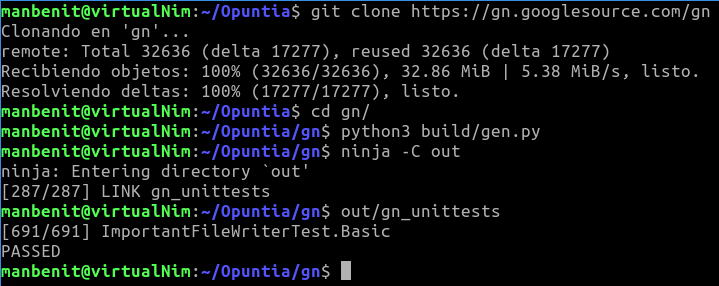
\includegraphics[scale=0.4]{installGn.png}
	\end{center}
\end{frame}

\begin{frame}{Instalación de LLVM}
	\begin{center}
		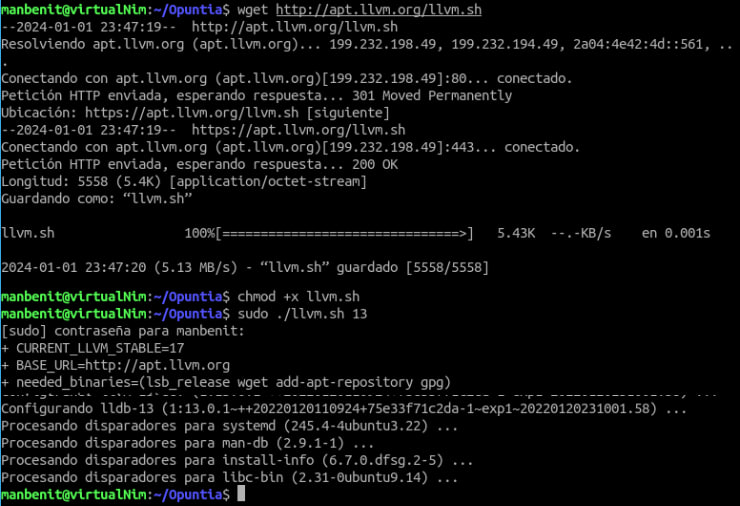
\includegraphics[scale=0.5]{installLlvm.jpg}
	\end{center}
\end{frame}

\begin{frame}{Instalación del \textit{toolchain} para x86}
	\begin{center}
		\ttfamily
		chmod 775 toolchains/scripts/i686-elf-tools.sh
		
		\enter
		
		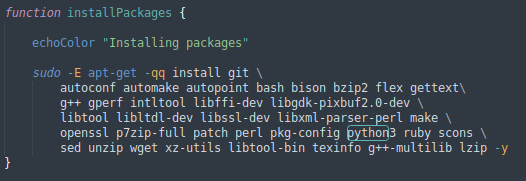
\includegraphics[scale=0.55]{modificarPython.png}
		
		\enter
		
		./toolchains/scripts/i686-elf-tools.sh
	\end{center}
\end{frame}

\begin{frame}{Instalación del \textit{toolchain} para x86}
	\begin{center}
		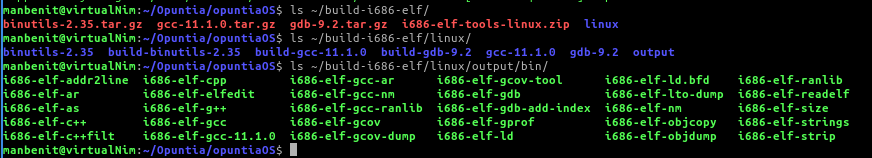
\includegraphics[scale=0.35]{toolchainx86_res.png}
		
		\enter
		
		\ttfamily
		export PATH=\$PATH:<directorio\_de\_contrucción>/linux/output/bin
	\end{center}
\end{frame}


\begin{frame}{Instalación de \textit{toolchain} para ARM}
	\begin{center}
		\ttfamily
		chmod 775 toolchains/scripts/arm-none-eabi-tools.sh
		
		\enter
		
		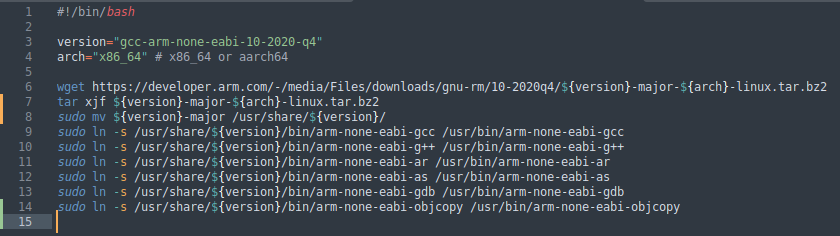
\includegraphics[scale=0.35]{modifArmSsh.png}
		
		\enter
		
		./toolchains/scripts/arm-none-eabi-tools.sh
	\end{center}
\end{frame}

\begin{frame}{Instalación del \textit{toolchain} para ARM}
	\begin{center}
		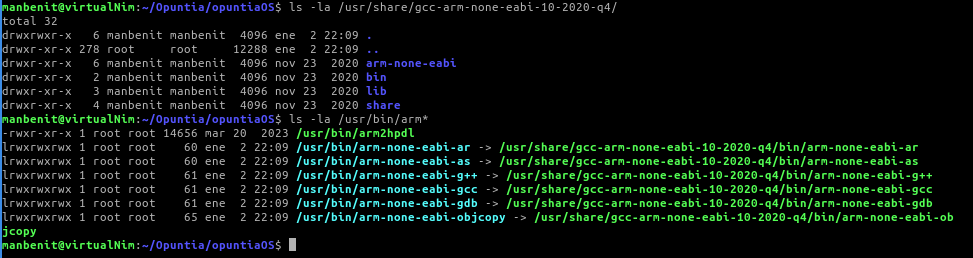
\includegraphics[scale=0.3]{toolchainArm_res.png}
	\end{center}
\end{frame}



%\section{Contrucción}

\section{Análisis}
\begin{frame}{}
	
\end{frame}

\begin{frame}{Implementación del \textit{bootloader}}
	Lo primero de lo que es posible percatarse al analizar la implementación del \textit{bootloader} es que la estructura de carpetas y archivos es distinta para \texttt{ARM} y \texttt{x86}.
	\begin{center}
		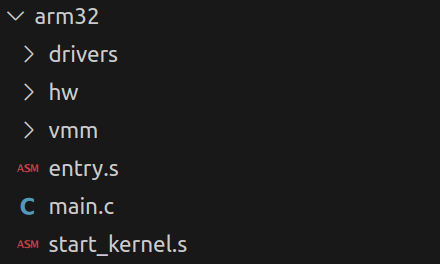
\includegraphics[scale=0.3]{estrucDir_ARM.png}
		\hspace{0.5cm}
		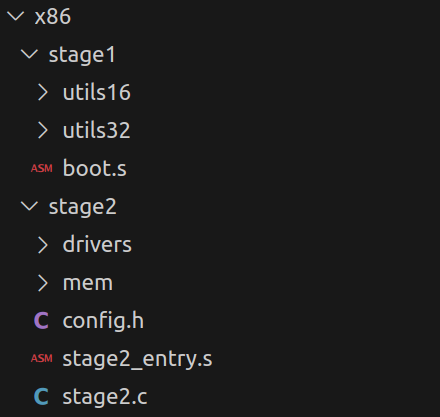
\includegraphics[scale=0.3]{estrucDir_x86.png}
	\end{center}
\end{frame}

\begin{frame}{Implementación del \textit{bootloader}}
	En el caso de \texttt{OpuntiaOS} para \texttt{x86}, se manejan 2 archivos de etapa para el arranque del sistema en lugar de 1, es decir, no se generará el archivo \texttt{stage2\_eltorito}, si no que se generarán 2 archivos de carga de \textit{kernel}.
	\begin{center}
		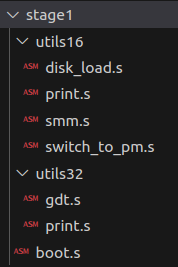
\includegraphics[scale=0.3]{x86_stage1_code.png}
		\hspace{0.5cm}
		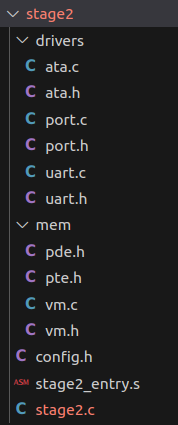
\includegraphics[scale=0.3]{x86_stage2_code.png}
	\end{center}
\end{frame}

\begin{frame}{}
	La primera etapa de carga contiene solo código ensamblador, es to es porque \texttt{stage1} se carga desde la BIOS y es la encargado de realizar la primera carga del \textit{kernel}, se puede decir que el archivo más importante es \texttt{boot.s}, similar a los \textit{kernel} compilados en el curso.
\end{frame}


\begin{frame}{Implementación del \textit{bootloader}}
	En el caso de \texttt{OpuntiaOS} para \texttt{ARM}, el \textit{bootloader} trabaja en 2 etapas, la primera en modo supervisor, que se encarga de acceder a los recursos del sistema y poder ejecutar el \textit{kernel} del sistema y la de modo usuario, donde se restringe el acceso a \textit{hardware}.
	\begin{center}
		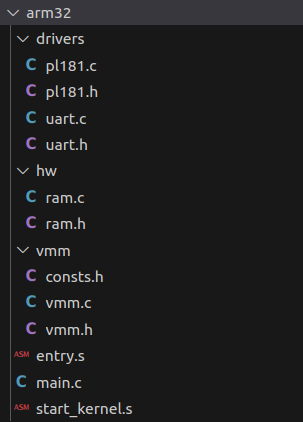
\includegraphics[scale=0.3]{arm_boot_code.png}
	\end{center}
\end{frame}

\begin{frame}{}
	La primera etapa de carga contiene solo código ensamblador, es to es porque \texttt{stage1} se carga desde la BIOS y es la encargado de realizar la primera carga del \textit{kernel}, se puede decir que el archivo más importante es \texttt{boot.s}, similar a los \textit{kernel} compilados en el curso.
\end{frame}





	\section{Conclusiones}
\begin{frame}
	Se logró compilar exitosamente el \textit{kernel} de \texttt{OpuntiaOS} para
	las arquitecturas \texttt{ARM} y \texttt{x86}, utilizando el código de su repositorio.
	
	\enter
	
	Se logró emular, con ayuda de la herramienta \texttt{QEMU}, el sistema
	\texttt{OpuntiaOS} bajo las arquitecturas \texttt{ARM} y \texttt{x86}.
	
	\enter
	
	Fue posible comprender el funcionamiento del \textit{bootloader} de \texttt{OpuntiaOS} para el correcto arranque del sistema para las arquitecturas \texttt{ARM} y \texttt{x86}.
	
	\enter
	
	Se compararon lo puntos principales del arranque de ambas arquitecturas, teniendo en cuenta los modos que ambos manejan para dar control al sistema operativo.
\end{frame}


\begin{frame}
	Se tuvieron dificultades al arrancar el sistema en máquinas reales, se tiene la emulación con ayuda de \texttt{QEMU}.
	
	\enter
	
	Se hizo una relación de las estructuras de datos, así como de la estructura de los archivos fuente del \textit{kernel} de \texttt{OpuntiaOS} con aquellos respectivos vistos en el curso.
	
	\enter
	
	Finalmente, pese a que no fue posible ver \texttt{OpuntiaOS} fincionando en una máquina real, se comprendió su funcionamiento.
	
\end{frame}
\end{document}
%\end{comment}





